\section{OMNIFORE: FRAMEWORK FOR OPTIMIZATION OF RESOURCE FORECASTS IN EDGE-CLOUD NETWORKS}
\label{sec: Proposed Solution}
%\section{OmniFORE: Framework for Optimization of Resource Forecasts in Edge-cloud Networks}

OmniFORE brings together several important innovations: a highly efficient attention mechanism, a strategic method for sampling data, advanced techniques for clustering time-series data, hyperparameter optimization, and scaling strategies to handle large numbers of traces.

\subsection{Trace Sampling Strategy}
\label{sec: Trace Sampling Strategy}


\begin{figure}
\centering
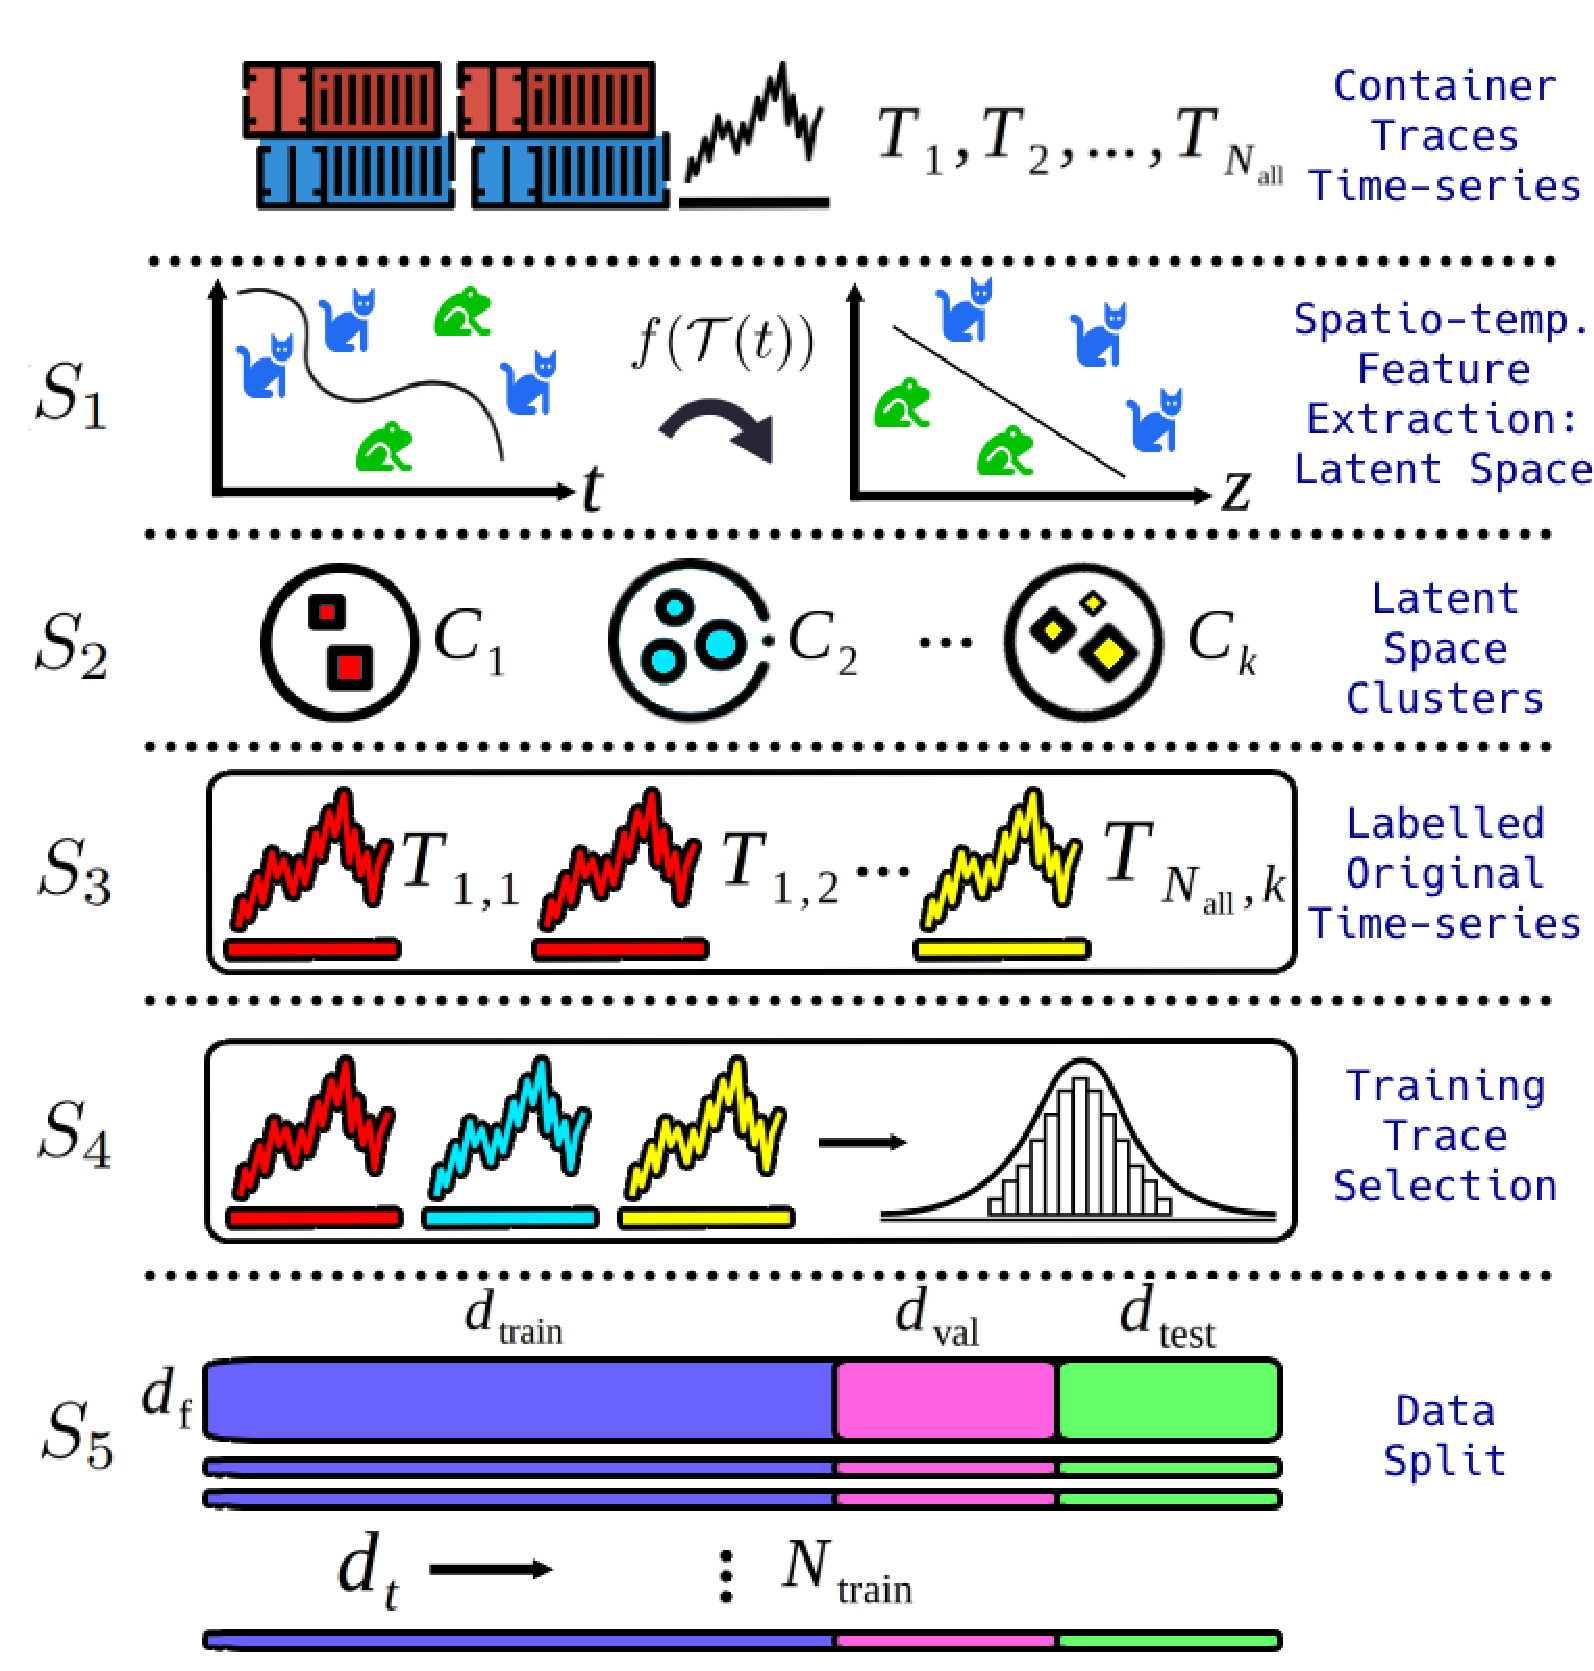
\includegraphics[width=0.49\textwidth]{img/proposed_solution_trace_selection.pdf}
\caption{Trace sampling process for generalization training. Historical workload data is processed to extract container traces, which are clustered into representative groups.}
\label{fig:proposed_solution_trace_selection}
\end{figure}

To achieve robust generalization across diverse workloads, OmniFORE employs a novel approach to extract a representative set of historical traces from the edge-cloud network. This strategy ensures that the model trained on these traces can effectively generalize to various workload types. The detailed steps ($S_1$ - $S_5$) of this process are outlined in Fig. ~\ref{fig:proposed_solution_trace_selection}.

The goal of these steps is to extract a \textbf{set of historical traces}, denoted as \(\mathbf{T}_{\text{train}}(t)\), where \(N_{\text{train}}\) represents the number of training traces. This set is a representative subset of the entire set of traces, \(\mathbf{T}_{\text{all}}(t)\), which contains \(N_{\text{all}}\) traces. "Representative" means that \(\mathbf{T}_{\text{train}}(t)\) captures the essential characteristics and variations present in \(\mathbf{T}_{\text{all}}(t)\), ensuring that the training set accurately reflects the diversity and distribution of the full dataset:

\begin{equation}
\mathbf{T}_{\text{train}}(t) \in \mathbb{R}^{d_f \times d_t \times N_{\text{train}}} \subset \mathbf{T}_{\text{all}}(t) \in \mathbb{R}^{d_f \times d_t \times N_{\text{all}}},
\end{equation}
where $N_{\text{train}} < N_{\text{all}}$. Using all traces for training would be computationally prohibitive and costly.

Section \ref{sec: Container Trace Heterogeneity} underscores the diverse workloads handled by containers, which require efficient resource management through OmniFORE. The highly dynamic nature of container data, marked by their time-dependent spatio-temporal patterns, presents significant challenges for analysis. Traditional clustering algorithms often struggle with such complex time-series data \cite{gupta2020approaches}. To overcome this, we propose transforming the data into a latent space to create a dense representation, facilitating more efficient clustering and differentiation \cite{frazier2018tutorial}. This latent space captures essential features, enabling better management of the data's complexities.

First ($S_1$), OmniFORE extracts spatio-temporal features from the container trace time-space, denoted as $\mathcal{T}$. Each trace $T_i(t) \in \mathbb{R}^{d_f \times d_{\text{t}}}$ is then transformed into \textbf{a lower-dimensional latent space}, $\mathcal{Z} \in \mathbb{R}^{z}$, where $z \ll d_f \times d_t$. This transformation, defined as $\mathcal{Z}(z) = f_{\text{encoder}}(\mathcal{T}(t))$, is optimized to capture the essential spatio-temporal patterns of the data over time. Details are provided in Section \ref{sec: Unsupervised Temporal Clustering}. By converting the time-dependent space $\mathcal{T}$ into the latent space $\mathcal{Z}$, OmniFORE optimizes for the most informative features for clustering, enhancing both efficiency and effectiveness by reducing dimensionality while preserving essential temporal information.

Second ($S_2$), the latent space $\mathcal{Z}$ is then \textbf{clustered}. Each cluster $C_k$ groups all container traces with similar spatio-temporal patterns over time into $K$ groups. The clustering process can be represented as
\begin{equation}   
\{C_1, C_2, \ldots, C_K\} = \text{Cluster}(\mathcal{Z}(z)).
\end{equation}
Third ($S_3$), each cluster \(C_k\) labels the original time-series traces, preserving the unique characteristics of each trace for accurate model training while leveraging the efficiency of latent space clustering. This can be mathematically depicted as
\begin{equation}
\mathbf{T}_{\text{all, cluster}}(t) = \{T_{1,1}(t), T_{2,1}(t), \ldots, T_{N_\text{all},k}(t)\},
\end{equation}
where $T_{1,1}(t)$ indicates the first trace in cluster 1.

Fourth ($S_4$), \textbf{representative traces} from each cluster $C_k$ are selected for training the prediction model. The selection process is optimized to ensure that the training data is diverse and representative of the broader dataset. Given a total number of traces $N_{\text{all}}$ and a desired subset of $N_{\text{train}}$ traces, the selection process is proportional to the number of traces in each cluster.

Let $N_{C_k}$ denote the number of traces in cluster $C_k$. The proportion of traces in each cluster compared to the total number of traces is
\begin{equation}
p_k = \frac{N_{C_k}}{N_{\text{all}}} \in \left[ 0, 1 \right].
\end{equation}
The number of traces selected from each cluster $C_k$ for the training set is
\begin{equation}
N_{\text{train},k} = \left\lfloor p_k \cdot N_{\text{train}} \right\rfloor,
\end{equation}
where $N_{\text{train},k}$ is the number of traces selected from cluster $C_k$ for training.

Therefore, the total number of traces in the training set $T_{\text{train}}$ is the sum of the selected traces from each cluster, such that

\begin{equation}  
N_{\text{train}} = \sum_{k=1}^{K} N_{\text{train},k}.
\end{equation}

%% data split
Finally ($S_5$), the traces in the sampled training set are split into train/validation/test segments along the time dimension ($d_t = d_{\text{train}} + d_{\text{val}} + d_{\text{test}}$), resulting in:

\begin{equation}
\begin{aligned}
&\text{\textit{training set:}} \quad  & \mathbf{T}_{\text{train}} &\in \mathbb{R}^{d_{\text{train}} \times d_{\text{f}} \times N_{\text{train}}}, \\
&\text{\textit{validation set:}} \quad & \mathbf{T}_{\text{val}} &\in \mathbb{R}^{d_{\text{val}} \times d_{\text{f}} \times N_{\text{train}}}, \\
&\text{\textit{test set:}} \quad & \mathbf{T}_{\text{test}} &\in \mathbb{R}^{d_{\text{test}} \times d_{\text{f}} \times N_{\text{train}}}.
\end{aligned} 
\end{equation}

OmniFORE ensures that data is effectively utilized for training, validating, and testing the prediction models, resulting in robust and generalizable performance.

\subsection{Unsupervised Temporal Clustering}
\label{sec: Unsupervised Temporal Clustering}

Figure \ref{fig:latent_space_creation} provides an overview of the \textbf{latent space extractor}. The input time-series $\mathcal{T}(t)$ is transformed into a latent space $\mathcal{Z}(z)$ by the encoder function $f_{\text{encoder}}$. The decoder function $f_{\text{decoder}}$ then reconstructs $\mathcal{Z}(z)$ into the output time-series $\mathcal{R}(t)$, which approximates $\mathcal{T}(t)$. This neural network structure compresses the data into a latent space, captures its critical features, and then reconstructs the original data. Successful reconstruction with the latent space acting as a \textbf{bottleneck} indicates that the latent space effectively encapsulates the essential information of the input signal.

To utilize this dense representation, we modify a \textbf{supervised} (using correct cluster labels for each trace) CNN-based approach for time-series clustering from \cite{clusteringDL} to an \textbf{unsupervised} (without cluster labels) version within OmniFORE. This process involves feature extraction through convolutional and pooling operations on raw data, followed by clustering in the latent space.

% Fig. \ref{fig:2d_latent_space} shows a 2D Principal Component Analysis \cite{abdi2010principal} of clusters in the latent space, where each point represents a time-series trace, color-coded by cluster.

\begin{figure}
\centering
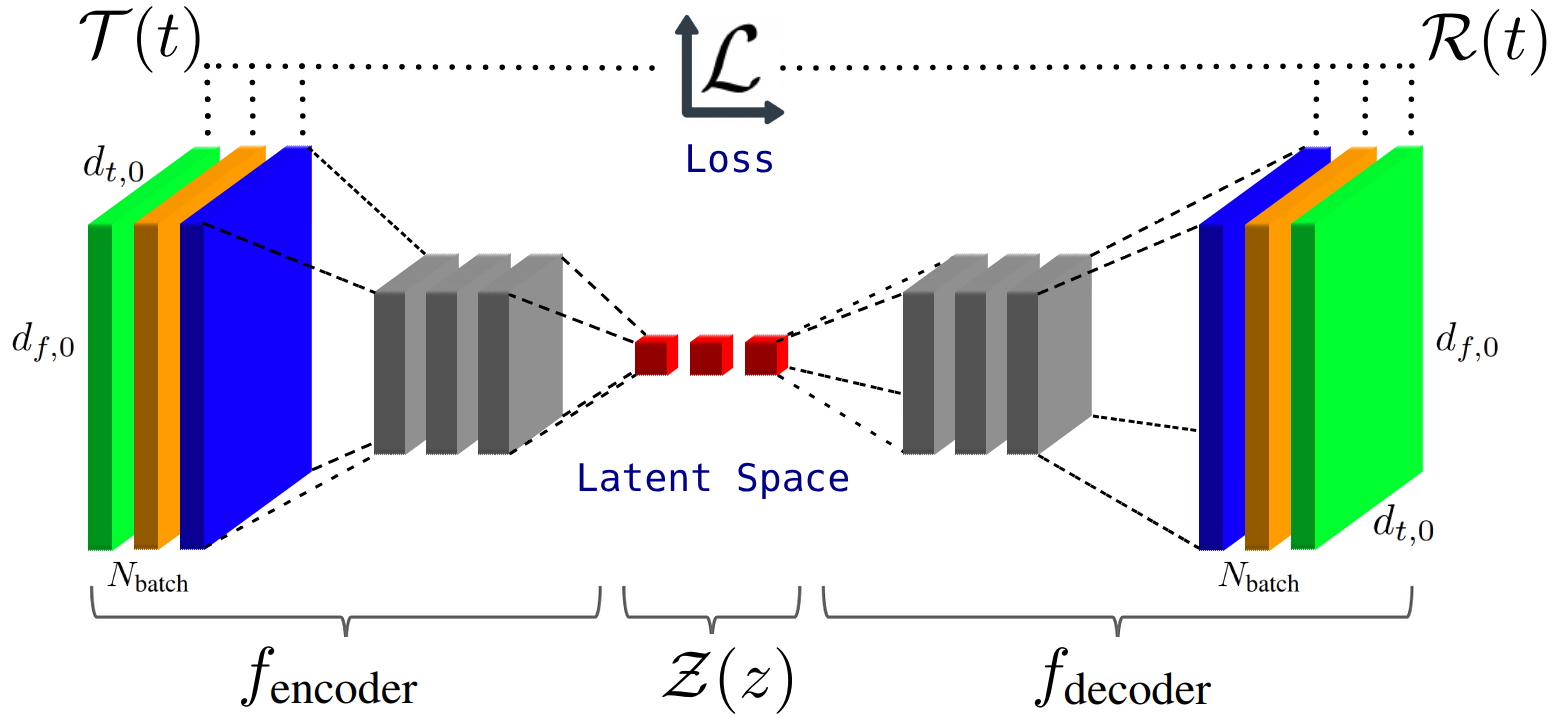
\includegraphics[width=0.49\textwidth]{img/latent_space_creation.png}
\caption{Overview of the latent space extractor. The input $\mathcal{T}(t)$ is encoded into latent space $\mathcal{Z}(z)$ by $f_{\text{encoder}}$ and then decoded by $f_{\text{decoder}}$ to reconstruct $\mathcal{R}(t) \approx \mathcal{T}(t)$.}
\label{fig:latent_space_creation}
\end{figure}

The architecture of the latent space extractor comprises the following layers:
\begin{enumerate}
    \item \textbf{Encoder}: Transforms an input trace $T_i$ into the latent space $\mathcal{Z}(z)$ using $\mathcal{Z}(z) = f_{\text{encoder}}(\mathcal{T}(t))$.
    \begin{itemize}
        \item \textbf{Input Layer}: \(d_{f,0} \times d_{t,0}\) neurons, where \(d_{t,0}\) is the series length and \(d_{f,0}\) is the number of features.
        \item Several repetitions \(r\) of combined convolutional and pooling layers, where \(d_{f,r}\) is the number of filters and \(d_{t,r}\) is the size of the sequence dimension after the \(r\)-th convolutional layer. The transformed sequence is \(T'(t') \in \mathbb{R}^{d_{f,r} \times d_{t,r} \times N_{\text{all}}}\).
        \begin{itemize}
            \item \textbf{Convolutional Layers ${\boldsymbol{C}}_{r}(t')$}: Parameters are convolution stride ($s_r$), filter size ($d_{f,r-1} \times l_r$), activation functions, trainable weights ($\boldsymbol{\omega}_r$), and biases ($\boldsymbol{b}_r$).
            \item \textbf{Pooling Layers $\boldsymbol{P}_r(t')$}: Downsampling strategy to reduce feature map size by averaging regions.
        \end{itemize}
        \item \textbf{Latent Space Layer}: Converts the flattened output of the last convolutional layers, $\boldsymbol{C}_r$, into a lower-dimensional latent space, $\mathcal{Z} \in \mathbb{R}^{z \times N_{\text{batch}}}$, where $z \ll d_{f,0} \times d_{t, 0}$.
    \end{itemize}
    \item \textbf{Decoder}: Converts $\mathcal{Z}(z)$ back to $\mathcal{T}(t)$ as $\mathcal{R}(t) = f_{\text{decoder}}(\mathcal{Z}(z)) \approx f_{\text{encoder}}^{-1}(\mathcal{Z}(z))$.
        \begin{itemize}
            \item \textbf{Multiple Transposed Convolution Layers}: Reconstruct the time-series input data from the latent representation, back to the original data shape. Transposed convolutions, also known as deconvolutions, upsample the input by reversing the operations of standard convolutional layers.
        \end{itemize}
\end{enumerate}
The training process can be described as:
\begin{enumerate}
    \item \textbf{Initialize}: Set up the Encoder-Decoder architecture, initialize weights and biases.
    \item \textbf{Load Input Data}: Prepare input traces as $\mathbf{T_{\text{all}}} \in \mathbb{R}^{ d_{t,0} \times d_{f,0} \times N_{\text{all}}}$, split into $N_{\text{batch}}$ batches. Here, $N_{\text{batch}}$ denotes the number of batches.
    \item \textbf{Forward Pass}: Compute the output of each layer for each batch.
    
    \begin{itemize}
        \item \textbf{Encoder Convolution Layer}:
        \begin{footnotesize}
        \begin{equation}
        \boldsymbol{C}_r(t') = \sum_{i=1}^{l_r} \sum_{j=1}^{d_{f, r-1}} T^{'}_R(i+s_r(t'-1), j) \boldsymbol{\omega}_r(i, j) + \boldsymbol{b}(r),
        \end{equation}
        \end{footnotesize}
        where $\boldsymbol{\omega}_r \in \mathbb{R}^{l_r \times d_f}$ and $\boldsymbol{b}(r)$ are the weights and bias of the $r$-th convolution filter.
        
        \item \textbf{Encoder Pooling Layer}:
        \begin{footnotesize}
        \begin{equation}
        \boldsymbol{P}_r(t') = \operatorname{MaxPool}\left(\boldsymbol{C}_r((t'-1)l_r+1), \ldots, \boldsymbol{C}_r(t' l_r)\right).
        \end{equation}
        \end{footnotesize}
        \item \textbf{Decoder}: Transposed convolutions for reconstruction.
    \end{itemize}
    \item \textbf{Loss Function}: Calculate the mean-square error across all batches between the reconstructed time-series and the actual input time-series as
    \begin{equation}
    \mathcal{L} = \frac{1}{2N_{\text{batch}}} \sum_{n=1}^{N_{\text{batch}}} \sum_{t=1}^{d_t} \Big(T_i(t) - R_i(t) \Big)^2.
    \end{equation}
    \item \textbf{Update}: Use gradient descent to update the weights and biases of the (transposed) convolutions ($\boldsymbol{\omega}_r$, $\boldsymbol{b}_r$) and optimize for minimizing the loss function.
    \item \textbf{Iterate}: Repeat with new batches until the model converges.
\end{enumerate}


\subsection{Fast Attention Mechanism for Extended Sequences}

The original transformer model \cite{vaswani2017attention} significantly enhances dependency capture, yet faces computational hurdles with long sequences \cite{wen2022transformers}. Recent developments in efficient transformers \cite{fasterandlightertransformers} and sparse attention techniques \cite{gorbett2023sparse, STRec, ma2024multivariate} mitigate these issues. Within OmniFORE, we enhance informers \cite{zhou2021informer}, which leverage sparse attention mechanisms to predict extensive time-series data efficiently. This optimization makes informers a viable alternative to traditional transformers, despite their implementation complexity, and a crucial element of our proposed solution.

The original self-attention mechanism \cite{vaswani2017attention} is defined by

\begin{equation}
\mathcal{A}(\mathbf{Q}, \mathbf{K}, \mathbf{V}) = \operatorname{Softmax}\left(\frac{\mathbf{QK}^\top}{\sqrt{d_{\text{embed}}}}\right) \mathbf{V},
\end{equation}
where $\mathbf{Q}, \mathbf{K}, \mathbf{V} \in \mathbb{R}^{d_x \times d_{\text{embed}}}$ are the query, key, and value matrices, respectively, while $d_{\text{embed}}$ is the embedding dimension of each point in the input sequence of length $d_x$. The product $\mathbf{QK}^\top \in \mathbb{R}^{d_x \times d_x}$ measures the importance of relationships between every data point in the sequence. This attention mechanism has $\mathcal{O}(d_x^2)$ complexity, making it inefficient for long input sequences.

The architectural innovations of informers compared to the original transformer can be summarized as follows:

\subsubsection*{\textbf{$\text{Informer}^{+1}$: Computationally Efficient Attention}}

The sparse self-attention mechanism enhances efficiency by concentrating on the most critical queries. This is done by forming a sparse matrix $\overline{\mathbf{Q}}$ that retains only the essential queries from $\mathbf{Q}$, with other entries set to zero. The selection of these important queries is directed by a sparsity measurement \cite{zhou2021informer}. This method significantly reduces computational complexity, making it more suitable for long sequences, as it scales linearly with the natural logarithm of the sequence length: $\mathcal{O}(d_x \log d_x)$.

\subsubsection*{\textbf{$\text{Informer}^{+2}$: Memory Saving with Attention Distilling}}

Due to the presence of zeros in the input matrix $\overline{\mathbf{Q}}$, the attention matrix $\mathcal{A}$ contains unnecessary entries. Removing these superfluous entries conserves memory and enables the model to concentrate on significant entries, a process known as attention distilling.

In each attention layer, the encoder utilizes self-attention distilling to minimize memory consumption by emphasizing the dominant entries in the attention matrix, thereby generating a new matrix

\begin{equation}
\mathcal{A}_{\text{distil}} = \operatorname{MaxPool}\left(\operatorname{ELU}\left(\operatorname{Conv1d}\left(\mathcal{A}\right)\right)\right),
\end{equation}

where $\operatorname{Conv1d}$ applies 1-D convolutional filters along the time dimension, and the activation function $\operatorname{ELU}$ \cite{al2023fhic} is used. The result is then passed through a max-pooling layer to downsample $\mathcal{A}$. This process decreases the time dimension of the input, reducing memory usage to $\mathcal{O}(d_x \log d_x)$.

\subsubsection*{\textbf{$\text{Informer}^{+3}$: Fast Inference}}

The decoder accelerates predictions for long sequences by utilizing generative inference, which forecasts the entire sequence in one step instead of predicting each time step sequentially. This is accomplished by using a known "start token" in conjunction with placeholders for the future sequence, formulated as

\begin{equation}
T_{\mathrm{de}}^{t} = \operatorname{Concat}\left(T_{\text{token}}^{t}, T_{\mathbf{0}}^{t}\right) \in \mathbb{R}^{(d_{\text{token}} + d_y) \times d_{\text{embed}}},
\end{equation}

where $T_{\text{token}}^{t} \in \mathbb{R}^{d_{\text{token}} \times d_{\text{embed}}}$ is the start token, and $T_{\mathbf{0}}^{t} \in \mathbb{R}^{d_y \times d_{\text{embed}}}$ acts as a placeholder for the future sequence. This generative inference approach significantly reduces computation time while preserving accuracy.



\subsection{Scaling}

Container traces in edge-cloud computing exhibit significant variability in resource usage, necessitating individual normalization to ensure balanced training. OmniFORE normalizes each trace such that the mean of the metric under study is zero (i.e., $\mu_i=0$) and the variance is one (i.e., $\sigma_i^2=1$), thereby preventing traces with higher means and variances from overshadowing others and enhancing model generalization.

Given a training set $\mathbf{T_{\text{train}}} \in \mathbb{R}^{d_t \times d_{\text{f}} \times N_{\text{train}}}$, each trace $T_i(t)$ is normalized as follows:

\begin{equation}
\tilde{T}_i(t) = \frac{T_i(t) - \mu_i}{\sigma_i},  
\end{equation}
where $\tilde{T}_i(t)$ denotes the normalized version of the trace $T_i(t)$, \(\mu_i\) is the mean, and \(\sigma_i = \sqrt{\sigma_i^2}\) is the standard deviation of the \(i\)-th trace. The mean \(\mu_i\) and variance \(\sigma_i^2\) are calculated as:

\begin{equation}
\mu_i = \frac{1}{d_t} \sum_{t=1}^{d_t} T_i(t), \quad \sigma_i^2 = \frac{1}{d_t} \sum_{t=1}^{d_t} (T_i(t) - \mu_i)^2.
\end{equation}

The scaling parameters $(\mu_i, \sigma_i^2)$ are saved for each trace. During testing, these parameters are used to invert the normalization of predictions back to the original scale, such that:

\begin{equation}
\hat{T}_i(t) = \tilde{T}_i(t) \cdot \sigma_i + \mu_i,
\end{equation}
where $i$ indexes each trace to maintain the scaling parameters for each trace.

\subsection{Bayesian Optimization with Generalization Objective}
\label{sec: Bayesian Optimization with Generalization Objective}

Optimizing hyperparameters is essential for improving model performance and generalization \cite{hyperparamsdatasets}. Due to the impracticality of traditional grid search in expansive hyperparameter spaces \cite{gridsearchvsbayesian}, Bayesian optimization \cite{frazier2018tutorial} offers an efficient alternative by constructing a probabilistic model of the objective function and iteratively selecting the most promising hyperparameters.

Figure \ref{fig:gp_toy_example} illustrates Bayesian optimization, starting with initial observations (red dots) of the objective function. This simplified example reduces the hyperparameter space to prediction length $d_y$, though in practice it is multidimensional (hyperparameter vector $\mathbf{h}$). A model (blue line) predicts the objective function's mean and confidence interval (CI, shaded area). The next hyperparameter (star) is selected based on predicted high performance and uncertainty, balancing exploration and exploitation.

OmniFORE's custom objective function $\text{Obj}(\mathbf{h})$ aims to maximize generalization across diverse container traces:
\begin{equation}
    \text{Obj}(\mathbf{h}) = \frac{1}{N_{\text{val}}} \sum_{i=1}^{N_{\text{val}}} \text{Perf}(\mathbf{h}, T_{\text{val}, i}),
\end{equation}
where $N_{\text{val}}$ is the number of validation traces, $T_{\text{val}, i}$ is the $i$-th validation trace, and $\text{Perf}(\mathbf{h}, T_{\text{val}, i})$ represents the performance metric.

\begin{figure}
\centering
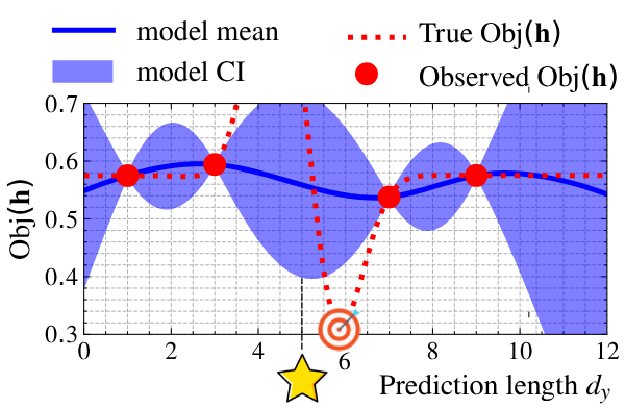
\includegraphics[width=0.49\textwidth]{img/gp_toy_example.pdf}
\caption{Bayesian optimization toy example. The star indicates the next value to try ($d_y = 5$). The target signifies the goal of minimizing the objective function.}
\label{fig:gp_toy_example}
\end{figure}
